\clearpage
%//==============================--@--==============================//%
%\vspace{-1em}
\subsection{P3 | Probabilidade de estar no estado 4 ao longo das sucessivas jogadas.}
\label{subsec:P3}
A evolução da probabilidade do estado $4$ é avaliada para um valor fixo de \textit{Njogadas} (50) e um valor sucessivamente maior de \textit{runs} de Monte Carlo:

\begin{figure}[ht] 
    \begin{subfigure}[b]{0.5\linewidth}
        \centering
        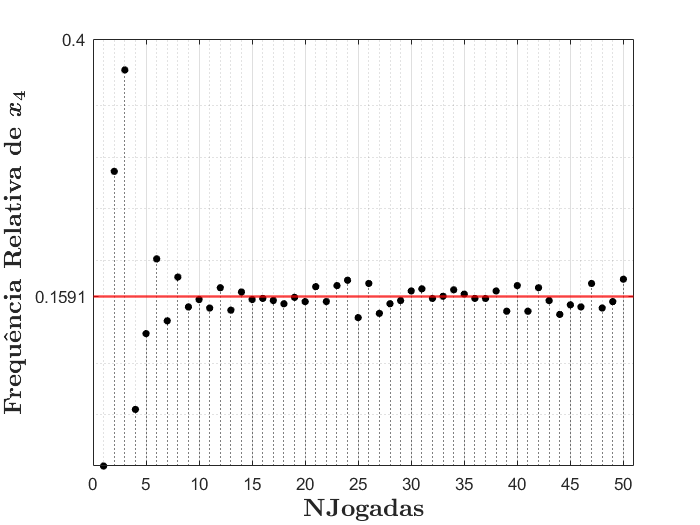
\includegraphics[width=1\linewidth]{img/P3/P31000.png}
        \caption{NMC = 1000} 
        \label{fig:P31000} 
        \vspace{1ex}
    \end{subfigure}%% 
    \begin{subfigure}[b]{0.5\linewidth}
        \centering
        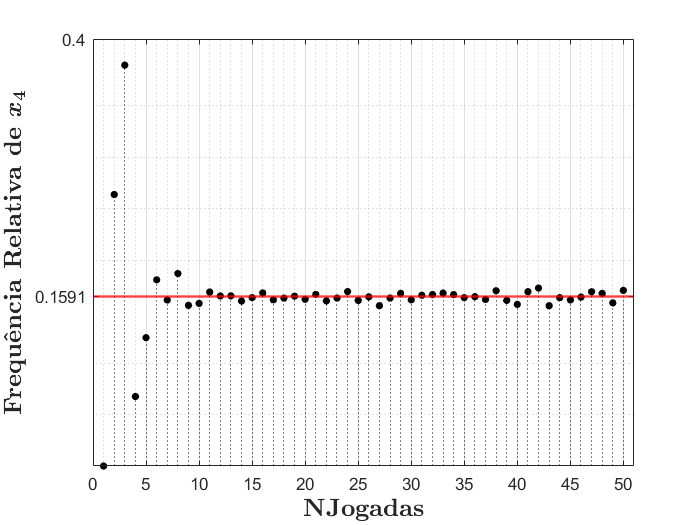
\includegraphics[width=1\linewidth]{img/P3/P310000.png} 
        \caption{NMC = 10000} 
        \label{fig:P310000} 
        \vspace{1ex}
    \end{subfigure} 
    \begin{subfigure}[b]{0.5\linewidth}
        \centering
        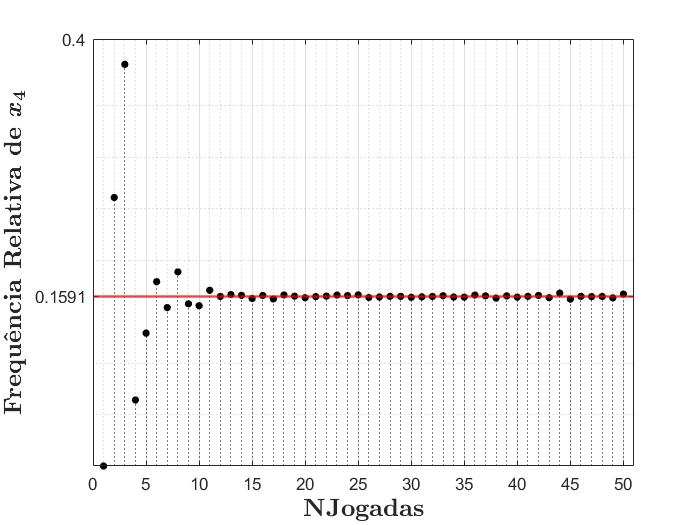
\includegraphics[width=1\linewidth]{img/P3/P3100000.png}
        \caption{NMC = 100000} 
        \label{fig:P3100000} 
        %%\vspace{4ex}
    \end{subfigure}%% 
    \begin{subfigure}[b]{0.5\linewidth}
        \centering
        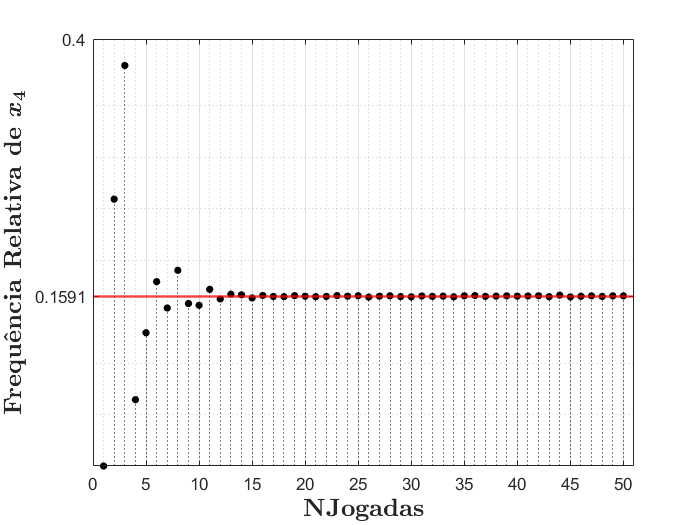
\includegraphics[width=1\linewidth]{img/P3/P31000000.png} 
        \caption{NMC = 1000000} 
        \label{fig:P31000000} 
        %%\vspace{4ex}
    \end{subfigure} 
    \caption{Evolução da probabilidade do estado $4$}
    \label{fig:LABEL}
\end{figure}

\noindent\textbf{\textit{$\rightarrow$ Observações}}

\begin{itemize}
    \item[$\blacktriangle$] Para a primeira jogada a probabilidade de estar no estado 4 é sempre nula, condição imposta pela casa de partida (apenas é possível transitar para o estado 1 ou 2).
    
    \item[$\blacktriangle$] A convergência da probabilidade para o seu \textit{steady-state value} é tanto mais rápida e mais exata quanto maior for o número de \textit{runs} de Monte Carlo (relembramos o \textit{convergence rate} de $\mathcal{O}(1/\sqrt{N})$, vide \hyperref[subsubsec:P2ii]{secção P2 ii)}.
    
     \item[$\blacktriangle$] O número de \textit{Njogadas} não necessita de ser muito grande para atingir uma boa estimativa do \textit{steady-state value}, sendo o número de \textit{runs} o parâmetro de maior peso nesta tarefa, reforçando novamente o uso de \textit{Many short runs}.
\end{itemize}

%//==============================--@--==============================//%